% !TEX program = pdflatex
\documentclass[aspectratio=169]{beamer}
\usetheme{Madrid}
\usecolortheme{default}
\usepackage{tikz}

% Custom colors
\definecolor{myblue}{RGB}{0,114,178}
\definecolor{myorange}{RGB}{230,159,0}
\definecolor{mygreen}{RGB}{0,158,115}
\definecolor{myred}{RGB}{213,94,0}
\definecolor{mypurple}{RGB}{204,121,167}
\definecolor{mybrown}{RGB}{240,228,66}
\definecolor{mygray}{RGB}{189,189,189}

% Set colors
\setbeamercolor{title}{fg=white,bg=myblue}
\setbeamercolor{frametitle}{fg=white,bg=myblue}
\setbeamercolor{section title}{fg=white,bg=myblue}
\setbeamercolor{subsection title}{fg=white,bg=myorange}
\setbeamercolor{item}{fg=myblue}
\setbeamercolor{subitem}{fg=myorange}

% Remove navigation symbols
\setbeamertemplate{navigation symbols}{}

% Custom commands
\newcommand{\limx}[2]{\lim_{x \to #1} #2}

% Title page
\title{The Derivative and the Tangent Line}
\subtitle{Definition, Geometric Meaning, and Applications}
\author{Differential Calculus}
\date{}

\begin{document}

\begin{frame}
\titlepage
\end{frame}

\begin{frame}{Outline}
\tableofcontents
\end{frame}

\section{The Derivative: Definition}

\begin{frame}{What is the Derivative?}
\begin{itemize}
  \item The derivative measures how a function changes as its input changes.
  \item It is the "instantaneous rate of change" or the "slope of the tangent line" at a point.
\end{itemize}
\end{frame}

\begin{frame}{Definition of the Derivative}
\begin{block}{Limit Definition}
The derivative of $f(x)$ at $x=a$ is:
\[
  f'(a) = \lim_{h \to 0} \frac{f(a+h) - f(a)}{h}
\]
\end{block}
\begin{itemize}
  \item If this limit exists, $f$ is said to be differentiable at $a$.
  \item $f'(a)$ is also called the "slope of the tangent line" to $f$ at $x=a$.
\end{itemize}
\end{frame}

\begin{frame}{Alternate Notation}
\begin{itemize}
  \item $f'(x)$ (prime notation)
  \item $\frac{df}{dx}$ or $\frac{dy}{dx}$ (Leibniz notation)
  \item $D_x f(x)$ (operator notation)
\end{itemize}
\end{frame}

% 新增例题1:绝对值函数
\begin{frame}{Example 1: Derivative of $f(x) = |x|$ at $x=0$}
\textbf{Question:} Find the derivative of $f(x) = |x|$ at $x=0$ using the definition.
\end{frame}

\begin{frame}{Solution to Example 1}
\textbf{Solution:}
\\
\[
\begin{aligned}
  f'(0) &= \lim_{h \to 0} \frac{|0+h| - |0|}{h} = \lim_{h \to 0} \frac{|h|}{h} \\
  &\text{If } h>0, \ \frac{|h|}{h} = 1; \quad \text{If } h<0, \ \frac{|h|}{h} = -1 \\
  &\text{Left-hand limit: } \lim_{h \to 0^-} \frac{|h|}{h} = -1 \\
  &\text{Right-hand limit: } \lim_{h \to 0^+} \frac{|h|}{h} = 1 \\
  &\text{Since left and right limits are not equal, the derivative does not exist at } x=0.
\end{aligned}
\]
\textbf{结论:}$f(x)=|x|$ 在 $x=0$ 处不可导。
\end{frame}

\section{Geometric Meaning}

\begin{frame}{Secant Line and Tangent Line}
\begin{itemize}
  \item The secant line through $(a, f(a))$ and $(a+h, f(a+h))$ has slope $\frac{f(a+h)-f(a)}{h}$.
  \item As $h \to 0$, the secant line approaches the tangent line at $x=a$.
\end{itemize}
\end{frame}

\begin{frame}{Tangent Line Visualization}
\begin{center}
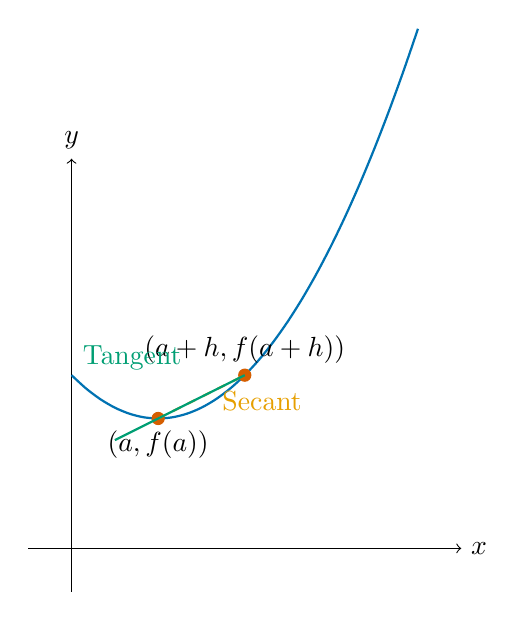
\begin{tikzpicture}[scale=1.1]
  % Axes
  \draw[->] (-0.5,0) -- (4.5,0) node[right] {$x$};
  \draw[->] (0,-0.5) -- (0,4.5) node[above] {$y$};
  % Curve
  \draw[domain=0:4,smooth,variable=\x,thick,color=myblue] plot ({\x},{0.5*\x*\x-\x+2});
  % Points
  \filldraw[myred] (1,1.5) circle (0.07);
  \filldraw[myred] (2,2) circle (0.07);
  % Secant line
  \draw[thick,dashed,color=myorange] (1,1.5) -- (2,2);
  % Tangent line at x=1
  \draw[thick,color=mygreen] (0.5,1.25) -- (2,2);
  % Labels
  \node at (1,1.2) {$(a, f(a))$};
  \node at (2,2.3) {$(a+h, f(a+h))$};
  \node[myorange] at (2.2,1.7) {Secant};
  \node[mygreen] at (0.7,2.2) {Tangent};
\end{tikzpicture}
\end{center}
\end{frame}

% 新增例题2:三次函数
\begin{frame}{Example 2: Derivative and Tangent Line for $f(x) = x^3$ at $x=1$}
\textbf{Question:} Find the derivative of $f(x) = x^3$ at $x=1$ and the equation of the tangent line.
\end{frame}

\begin{frame}{Solution to Example 2}
\textbf{Solution:}
\\
\[
\begin{aligned}
  f'(x) &= \lim_{h \to 0} \frac{(x+h)^3 - x^3}{h} \\
        &= \lim_{h \to 0} \frac{x^3 + 3x^2h + 3xh^2 + h^3 - x^3}{h} \\
        &= \lim_{h \to 0} \frac{3x^2h + 3xh^2 + h^3}{h} \\
        &= \lim_{h \to 0} (3x^2 + 3xh + h^2) = 3x^2 \\
  f'(1) &= 3(1)^2 = 3 \\
  f(1) &= 1^3 = 1 \\
  \text{Tangent line: } y &= f(1) + f'(1)(x-1) = 1 + 3(x-1)
\end{aligned}
\]
\end{frame}

\begin{frame}{Summary: Derivative and Tangent Line}
\begin{itemize}
  \item The derivative $f'(a)$ is the slope of the tangent line to $f$ at $x=a$.
  \item The tangent line at $x=a$ has equation:
  \[
    y = f(a) + f'(a)(x-a)
  \]
  \item The process of finding the derivative is called "differentiation".
\end{itemize}
\end{frame}

\section{Practice Problems}

\begin{frame}{Practice: 1 and 2}
\textbf{Practice 1:}
\[
\text{Find the derivative of } f(x) = x^2 
\]
\vspace{1em}
\textbf{Practice 2:}
\[
\text{Find the equation of the tangent line to } f(x) = x^2 \text{ at } x=1
\]
\end{frame}

% 新增练习题3-5
\begin{frame}{Practice: 3 and 4}
\textbf{Practice 3:}
\[
\text{Find the derivative of } f(x) = \sqrt{x} \text{ at } x=4
\]
\vspace{1em}
\textbf{Practice 4:}
\[
\text{Find the derivative of } f(x) = |x-2| \text{ at } x=2
\]
\end{frame}

\begin{frame}{Practice: 5}
\textbf{Practice 5:}
\[
\text{A particle moves along a line so that its position at time $t$ is } s(t) = t^2 - 4t + 5. \\
\text{Find the instantaneous velocity at } t=3.
\]
\end{frame}

\section{Solutions to Practice Problems}

\begin{frame}{Solution to Practice 1}
\textbf{Practice 1:}

Find the derivative of $f(x) = x^2$

\textbf{Solution:}
\[
\begin{aligned}
  f'(x) &= \lim_{h \to 0} \frac{(x + h)^2 - x^2}{h} \\
        &= \lim_{h \to 0} \frac{x^2 + 2xh + h^2 - x^2}{h} \\
        &= \lim_{h \to 0} \frac{2xh + h^2}{h} \\
        &= \lim_{h \to 0} (2x + h) = 2x
\end{aligned}
\]
\end{frame}

\begin{frame}{Solution to Practice 2}
\textbf{Practice 2:}

Find the equation of the tangent line to $f(x) = x^2$ at $x = 1$

\textbf{Solution:}
\[
\begin{aligned}
  f(1) &= 1^2 = 1 \\
  f'(x) &= 2x \implies f'(1) = 2 \\
  \text{Tangent line: } y &= f(1) + f'(1)(x-1) = 1 + 2(x-1)
\end{aligned}
\]
\end{frame}

% 新增解答3
\begin{frame}{Solution to Practice 3 (Part 1)}
\textbf{Practice 3:}

Find the derivative of $f(x) = \sqrt{x}$ at $x=4$

\textbf{Solution:}
\[
\begin{aligned}
  f'(x) &= \lim_{h \to 0} \frac{\sqrt{x+h} - \sqrt{x}}{h} \\
  &\text{Let } x=4: \\
  f'(4) &= \lim_{h \to 0} \frac{\sqrt{4+h} - 2}{h}
\end{aligned}
\]
\end{frame}

\begin{frame}{Solution to Practice 3 (Part 2)}
\textbf{Solution (continued):}
\[
\begin{aligned}
  &\text{Multiply numerator and denominator by } \sqrt{4+h} + 2: \\
  &= \lim_{h \to 0} \frac{(\sqrt{4+h} - 2)(\sqrt{4+h} + 2)}{h(\sqrt{4+h} + 2)} \\
  &= \lim_{h \to 0} \frac{4+h - 4}{h(\sqrt{4+h} + 2)} \\
  &= \lim_{h \to 0} \frac{h}{h(\sqrt{4+h} + 2)} \\
  &= \lim_{h \to 0} \frac{1}{\sqrt{4+h} + 2} = \frac{1}{4}
\end{aligned}
\]
\end{frame}

% 新增解答4
\begin{frame}{Solution to Practice 4 (Part 1)}
\textbf{Practice 4:}

Find the derivative of $f(x) = |x-2|$ at $x=2$

\textbf{Solution:}
\[
\begin{aligned}
  f'(2) &= \lim_{h \to 0} \frac{|2+h-2| - |2-2|}{h} \\
  &= \lim_{h \to 0} \frac{|h|}{h}
\end{aligned}
\]
\end{frame}

\begin{frame}{Solution to Practice 4 (Part 2)}
\textbf{Solution (continued):}
\[
\begin{aligned}
  &\text{If } h>0, \ \frac{|h|}{h} = 1 \\
  &\text{If } h<0, \ \frac{|h|}{h} = -1 \\
  &\text{Left-hand limit: } \lim_{h \to 0^-} \frac{|h|}{h} = -1 \\
  &\text{Right-hand limit: } \lim_{h \to 0^+} \frac{|h|}{h} = 1
\end{aligned}
\]
\end{frame}

\begin{frame}{Solution to Practice 4 (Part 3)}
\textbf{Solution (continued):}
\[
\begin{aligned}
  &\text{Since left and right limits are not equal,} \\
  &\text{the derivative does not exist at } x=2.
\end{aligned}
\]
\textbf{结论:}$f(x)=|x-2|$ 在 $x=2$ 处不可导。
\end{frame}

% 新增解答5
\begin{frame}{Solution to Practice 5 (Part 1)}
\textbf{Practice 5:}

A particle moves along a line so that its position at time $t$ is $s(t) = t^2 - 4t + 5$. Find the instantaneous velocity at $t=3$.

\textbf{Solution:}
\[
\begin{aligned}
  v(t) &= s'(t) = \lim_{h \to 0} \frac{s(t+h) - s(t)}{h} \\
  s'(t) &= \lim_{h \to 0} \frac{(t+h)^2 - 4(t+h) + 5 - (t^2 - 4t + 5)}{h}
\end{aligned}
\]
\end{frame}

\begin{frame}{Solution to Practice 5 (Part 2)}
\textbf{Solution (continued):}
\[
\begin{aligned}
  &= \lim_{h \to 0} \frac{t^2 + 2th + h^2 - 4t - 4h + 5 - t^2 + 4t - 5}{h} \\
  &= \lim_{h \to 0} \frac{2th + h^2 - 4h}{h} \\
  &= \lim_{h \to 0} (2t - 4 + h) = 2t - 4
\end{aligned}
\]
\end{frame}

\begin{frame}{Solution to Practice 5 (Part 3)}
\textbf{Solution (continued):}
\[
\begin{aligned}
  v(3) &= 2 \times 3 - 4 = 2
\end{aligned}
\]
\textbf{Answer:} The instantaneous velocity at $t=3$ is $2$ units/time.
\end{frame}

\end{document} 